

% arara: pdflatex: { synctex: yes }
% arara: makeindex: { style: ctuthesis }
% arara: bibtex

% The class takes all the key=value arguments that \ctusetup does,
% and a couple more: draft and oneside



\documentclass[twoside]{ctuthesis}

\ctusetup{
	%preprint = \ctuverlog,
%	mainlanguage = english,
%	titlelanguage = czech,
	mainlanguage = czech,
	otherlanguages = {english},
	title-czech = {Správa skautského oddílu},
	title-english = {Scout troop management},
	subtitle-czech = {Aplikace},
	subtitle-english = {Application},
	doctype = B,
	faculty = F3,
	department-czech = {Kabinet výuky informatiky},
	department-english = {Informatics teaching cabinet},
	author = {Patrik Kolář},
	supervisor = {Ing. Božena Mannová, Ph.D.},
	supervisor-address = {},
	supervisor-specialist = {},
	fieldofstudy-english = {Open Informatics},
	subfieldofstudy-english = {Computer Graphics},
	fieldofstudy-czech = {Otevřená informatika},
	subfieldofstudy-czech = {Počítačové hry a grafika},
	keywords-czech = {skauting, skaut, správa skautského oddílu},
	keywords-english = {scoot troop, scout troop management},
	day = 4,
	month = 11,
	year = 2024,
	specification-file = {},
%	front-specification = true,
	front-list-of-figures = false,
	front-list-of-tables = false,
%	monochrome = true,
%	layout-short = true,
}

\ctuprocess

\addto\ctucaptionsczech{%
	\def\supervisorname{Vedoucí}%
	\def\subfieldofstudyname{Studijní program}%
}

\ctutemplateset{maketitle twocolumn default}{
	\begin{twocolumnfrontmatterpage}
		\ctutemplate{twocolumn.thanks}
		\ctutemplate{twocolumn.declaration}
		\ctutemplate{twocolumn.abstract.in.titlelanguage}
		\ctutemplate{twocolumn.abstract.in.secondlanguage}
		\ctutemplate{twocolumn.tableofcontents}
		\ctutemplate{twocolumn.listoffigures}
	\end{twocolumnfrontmatterpage}
}

% Theorem declarations, this is the reasonable default, anybody can do what they wish.
% If you prefer theorems in italics rather than slanted, use \theoremstyle{plainit}
%\theoremstyle{plain}
%\newtheorem{theorem}{Theorem}[chapter]
%\newtheorem{corollary}[theorem]{Corollary}
%\newtheorem{lemma}[theorem]{Lemma}
%\newtheorem{proposition}[theorem]{Proposition}

%\theoremstyle{definition}
%\newtheorem{definition}[theorem]{Definition}
%\newtheorem{example}[theorem]{Example}
%\newtheorem{conjecture}[theorem]{Conjecture}

%\theoremstyle{note}
%\newtheorem*{remark*}{Remark}
%\newtheorem{remark}[theorem]{Remark}

\setlength{\parskip}{5ex plus 0.2ex minus 0.2ex}

% Abstract in Czech
\begin{abstract-czech}
Tato práce se zaměřuje na správu skautského oddílu, administrace členů, plánování akcí a kontrolování docházky skautů. Umožňuje také udělovat ocenění za splněné úkoly.
\end{abstract-czech}

% Abstract in English
\begin{abstract-english}
This bachelor's thesis focuses on the management of a Scout unit, including member administration, event planning, and attendance tracking for Scouts. It also provides the ability to grant awards for completed tasks.


\end{abstract-english}

% Acknowledgements / Podekovani
\begin{thanks}
Chtěl bych poděkovat všem, kteří mě během práce na tomto projektu podpořili, zejména vedoucí mé práce za cenné rady a inspiraci.
\end{thanks}

% Declaration / Prohlaseni
\begin{declaration}
Prohlašuji, že jsem tuto práci vypracoval samostatně a že jsem uvedl všechny použité zdroje v souladu s metodickými pokyny.

V Praze, \ctufield{day}.~\monthinlanguage{title}~\ctufield{year}
\end{declaration}



\begin{document}

\maketitle

\chapter{Úvod}
\section{Téma a cíl práce}
Cílem práce je vytvořit jednoduchou a přehlednou aplikaci jak pro vedoucí skautských oddílů, tak pro mladé skauty. Aplikace by měla sloužit pro administrativní potřeby a komunikaci mezi jednotlivými členy. Vedoucí tak budou moci vytvářet nové události a akce, zaznamenávat účast skautů a udělovat "bobříky".
\section{Skauting}
Skauting se poprvé objevil v Anglii v roce 1907, za jeho vznikem stál britský generál Robert Baden-Powell. O pár let později, roku 1912, proběhl první skautský tábor i v tehdejším Československu, který vedl Antonín Benjamín Svojsík. Zpočátku byl skauting určený pouze pro mladé chlapce, ale brzy se do skautských oddílů dostaly i dívky. \\

Skauti byli rozděleni do oddílů po menších počtech a každému oddílu byl navíc přiřazen starší a zkušenější jedinec. Hlavním významem tohoto sdružení byla výchova mládeže, naučit je čestnému chování, úctě k lidem, přírodě a sobě samým. \\

Později byly skauti rozděleni na starší a mladší oddíly pro zjednodušení organizace. Dnes je v Česku nejrozšířenější skautská organizace  "Junák – český skaut, z. s.".
\chapter{Seznámení s problematikou}
\section{Organizace}
Skautské sdružení může mít velké množství členů, a proto se rozdělují na různá střediska, kraje nebo oddíly. Každé sdružení může mít své vlastní rozdělení. Rozdílnost je také u sdružení v Česku a v zahraničí, tam může být celková struktura odlišná.

Na obrázku \ref{fig:rozdeleni} je vidět rozdělení Junáka - českého skauta. Tato organizace má více než 75 000 členů, a proto je potřeba rozsáhlejší dělení, a to je postupně podle krajů a následně okresů. V každém okresu pak existuje několik středisek a každé má pod sebou další oddíly. Výsledkem tohoto rozdělení je, že oddíl je například jedna vesnice, nebo několik blízkých vesnic a obsahuje kolem padesáti členů.
V americkém sdružení Boy Scouts of America to funguje lehce odlišně, zde jsou skauti rozděleni na Radu (council). Ten je nejnadřazenější skupinou a spravuje okresy jednotek. Jednotky jsou rozděleny podle věkových kategorií. Pro nejmladší skauty ve věku od 5 do 10 let je smečka (pack). Poté starší skauti od 11 do 17 let jsou v družině (troop). Výjimkou jsou kmeny (crew), které se zaměřují na speciální aktivity.

\begin{figure}[!ht]
\includegraphics[width=5in]{./images/rozdeleni_skautu.png}
\caption{Rozdělení Junáka - českého skauta}
\label{fig:rozdeleni}
\end{figure}

\section{Administrativa}
Z důvodu bezpečnosti a odpovědnosti za mladistvé si skautské sdružení uchovává určité informace o svých členech. Jsou to převážně osobní údaje jako jméno, datum narození, adresa nebo i rodné číslo pro pojišťovny. Dále jsou potřeba kontaktní informace na rodiče těchto mladých skautů, aby je v případě potřeby mohli vedoucí kontaktovat ohledně naléhavých situací. \\
Při velkém počtu informací si vedoucí nemůže pamatovat ani všechny zdravotní problémy ostatních, a proto se často zapisují i alergie, nemoci a užívané léky.

\chapter{Analýza existujících aplikací}


\section{SkautLS}
Oficiální aplikace Junáka - českého skauta. Jedná se o aplikaci zaměřenou především na administraci velkého počtu skautských oddílů, jednotek a jednotlivců. V aplikaci jsou skauti rozděleni do jednotek, které se stromově dělí podle krajů a následně samotných středisek.

Přední funkce této aplikace jsou hromadné rozesílání zpráv, a to i podřízeným střediskům. Dále také správa dotací mé jednotky a podřízených jednotek, pojištění odpovědnosti pro registrované členy a půjčování majetku a prostorů mezi oddíly. Nechybí zde ani vytváření akcí jako jsou výpravy nebo tábory.
Různé funkce jsou dostupné pouze pro určité role skautů a vedoucích. \\


\begin{itemize}
\setlength{\itemindent}{0.7cm}
    \item [\textbf{Výhody}]
    \item Organizace celého Junáka
    \item Správa financí
    \item Zdarma
    \item Česká aplikace
\end{itemize}


\begin{itemize}
\setlength{\itemindent}{1.1cm}
    \item [\textbf{Nevýhody}]
    \setlength{\itemindent}{0.7cm}
    \item Nepřehlednost
    \item Pouze základní funkce
\end{itemize}


\section{Levitio}
Jedná se o poměrně novou aplikaci z Ostravy. Nabízí přehled registrovaných členů, správu akcí s kalendářem, docházku a poměrně inovativní funkce jako tiskové šablony pro vyznamenání, karetní hry a podobné.

Aplikace také vede systém odznaků, úkolovník a virtuální nástěnku pro oddíly.
Je zde také možnost správy financí, přehledné zobrazení zaplacených poplatků za registrace, tábory a podobné. Bohužel si majitel účtuje provizi 3\% až 5\% z každé transakce pro další vývoj aplikace.

\begin{itemize}
\setlength{\itemindent}{0.7cm}
    \item [\textbf{Výhody}]
    \item Česká aplikace
    \item Systém odměn

\end{itemize}
\begin{itemize}
\setlength{\itemindent}{1.1cm}
    \item [\textbf{Nevýhody}]
    \setlength{\itemindent}{0.7cm}
    \item Provize ze všech transakcí
    \item Aplikace je ve vývoji
\end{itemize}


\section{TroopTrack}
Americká aplikace pro skauty po celém světě. Jako předchozí, i tato aplikace umožňuje rozdělení do oddílů a středisek. Také umožňuje plánovat akce, vedoucí mohou zaznamenávat docházku a udělovat odměny za splněné úkoly. Systém opět obsahuje více rolí pro správu systému. Součástí je také komunikační systém, který slouží jak mezi skauty, tak pro komunikaci s vedoucími. Umožňuje nahrávat soubory, fotografie a vytvářet profilovou stránku každého člena. Navíc obsahuje filtr pro nevyžádanou poštu, aby se zamezilo zneužívání zpráv.

Vedoucí mohou také spravovat finance svých oddílů, ukládat si účtenky a nechat si je zpětně proplácet. \\
Moderní zpracování aplikace dovoluje propojení s různými kalendáři a dalšími aplikacemi. Je dostupná jak na mobilních telefonech, tak ve webové aplikaci. Pokud to zařízení dovoluje, je možné propojit vstup do objektu pomocí čipových karet a zároveň zaznamenávat docházku.

Celý systém je v angličtině, což může být překážka pro různé členy oddílu. Další věc je cena aplikace, za její používání si prodejce účtuje 10 \$ měsíčně nebo 99 \$ ročně.

\begin{itemize}
\setlength{\itemindent}{0.7cm}
    \item [\textbf{Výhody}]
    \item Moderní a přehledné
    \item Propojení ostatních aplikací a kalendářů
    \item Správa financí
\end{itemize}
\begin{itemize}
\setlength{\itemindent}{1.1cm}
    \item [\textbf{Nevýhody}]
    \setlength{\itemindent}{0.7cm}
    \item Cena
    \item Bez podpory češtiny
\end{itemize}

\section{SCOUT BOOK}
Aplikaci vytvořila americká skupina "Boy Scouts of America (BSA)". Obsahuje podobné funkce jako předchozí aplikace, a to jsou administrace členů, plánování akcí, zasílání zpráv. Hlavní rozdíl je propracovaný systém vyznamenání a hodností, který skautům znázorňuje jejich postup.

Aplikace je stavěna pro mobilní zařízení, a to jak iOS, tak Android. To může být velkou výhodou pro přístup k aplikaci téměř kdekoli, kde se vyskytuje datové připojení. 

\begin{itemize}
\setlength{\itemindent}{0.7cm}
    \item [\textbf{Výhody}]
    \item Mobilní aplikace
    \item Odznaky a hodnocení
    \item Zdarma
\end{itemize}
\begin{itemize}
\setlength{\itemindent}{1.1cm}
    \item [\textbf{Nevýhody}]
    \setlength{\itemindent}{0.7cm}
    \item Bez podpory češtiny
    \item Systém pro Americký styl skautingu
\end{itemize}

\chapter{Specifikace}
V této kapitole jsou rozepsány klíčové vlastnosti a požadavky na aplikaci.
\section{Přehlednost}
Nejdůležitějším aspektem dobré aplikace je jednoduché používání aplikace a její přehlednost. Systém by neměl zobrazovat zbytečně moc informací, nabídky by neměli být příliš složité a rozsáhlé a v nejlepším případě by celá obrazovka měla minimalistický styl. \\
Z předem zmíněných aplikací je tento problém nejvíce vidět u aplikace SkautLS. Aby se zabránilo podobnému problému, bude tato aplikace rozdělena na více stránek. Tím se zabrání příliš mnoha informacím na jedné obrazovce a velmi to pomůže k vytvoření minimalistického designu. 

\section{Dostupnost} 
Velkou roli může také hrát cenová dostupnost. Sdružení skautů se vždy snažilo dělat nejvíce proto, aby mladým lidem poskytli spoustu zábavy, poznání a prožitků. Tyto věci mohou být finančně náročné a každé další peníze vynaložené na pouhou správu oddílu můžou být dostatečnou motivací pro zachování původního systému. \\
V dnešní době je spousta těchto aplikací měsíčně nebo ročně zpoplatněna. A to bez rozdílu, zda se jedná o malé středisko, které má 30 skautů, nebo velkou organizaci, kde jsou stovky členů. Po tomto zjištění zůstane tato aplikace zdarma přístupná všem skautským oddílům. \\
Určitě je potřeba zmínit ještě jazykovou dostupnost. Skautských aplikací v českém jazyce ještě moc neexistuje. To může být velká bariéra pro starší členy skautských oddílů nebo jejich vedoucí. Tato aplikace bude nativně psaná v češtině s podporou anglického překladu.

\section{Administrativa skautů} 
Předním důvodem pro změnu z papírových záznamů bývá velký problém s uchováním informací o všech členech oddílu, jejich osobních informacích, kontaktech na rodiče a dalších důležitých poznámkách například o nemocech nebo pravidelně užívaných lécích. \\
Uchovávání takového množství informací v digitální podobě není velký problém. Aplikace umožňuje uchovávat všechny tyto informace a především dodržet pravidla o ochraně osobních údajů. \\
Protože bude aplikace určena pro počítače ve skautských klubovnách, mohl by nastat problém, že by tyto informace nebyly dostupné někde na výletě. Skauti často chodí do přírody, kde nemusí být ani signál, a tak by nepomohla ani webová aplikace. Jako řešení tohoto problému se nabízí jednoduchý export dat do souboru PDF, který může mít vedoucí u sebe v mobilním zařízení nebo vytisknutý v papírové podobě.
\section{Plánování akcí} 
Systém pro plánování akcí a následné rozeslání je naprostou nutností této aplikace. Podobně jako u konkurenčních aplikací bude realizováno způsobem, že vedoucí oddílu nebo kdokoli s přidělenou rolí pro vytváření akcí bude mít možnost vytvořit událost a nechat ji automaticky rozeslat všem skautům, kterých se to týká. Skauti tak dostanou upozornění, že byli přidáni do akce a budou moci potvrdit účast a přečíst si všechny potřebné informace. Toto může pomoci předejít problému ohledně zapomínání akcí nebo nevědomosti z důvodu neúčasti na schůzkách.

%\section{Správa financí} \\
%TODO zjistit jak funguje

\section{Bobříky} 
Bobříky nebo vyznamenání za určité činy bývá velkou motivací pro spoustu skautů k dobrému a příkladnému chování. Prvních 13 bobříků se objevilo v knize Hoši od Bobří řeky (Jaroslav Foglar, 2005). Každé středisko si ovšem často vymýšlí své vlastní, podle možností a pravidelných aktivit. \\
Z tohoto důvodu bude aplikace obsahovat možnost vytvářet vlastní bobříky a udělovat je skautům za plnění různých aktivit.

\section{Další funkce} 
Některá střediska mají různé hodnosti pro skauty, podle jejich výsledků nebo věku. Čím dále postupují, dostávají větší privilegia nebo organizují různé akce. \\
Větší zahraniční aplikace jako je TroopTrack nebo Scoutbook nabízejí uživatelům využívat různá fóra nebo diskuzní články, sdílená úložiště pro nahrávání různých souborů nebo fotek a profilové galerie, kam si každý skaut může vystavit své největší úspěchy.

\section{Kompatibilita ostatních aplikací} 
Ostatní aplikace zřídka nabízejí i propojení s jinými aplikacemi. To může velmi usnadnit přesun ze starší platformy na novou. To ovšem může vést k domnění, že je aplikace naprosto zástupná té předchozí. Dále to také vyžaduje určité opatření z druhé strany, odkud by se data přesouvala.

\section{Podporované systémy} 
V dnešní době je asi nejrozšířenější rozhraní webové aplikace. Ta bývá přístupná jak na mobilním zařízení, tak na stolních počítačích. Velkou nevýhodou zde ale může být vyžadované připojení k internetu, které nemusí být vždy dostupné. \\
Aplikace čistě pro mobilní telefony se může zdát jako výborná volba, ale její vývoj a údržba už nemusí být tak jednoduchá, pokud chceme možnost jak pro Android, tak pro iOS. Často se každá verze musí vyvíjet zcela samostatně. \\
Následuje otázka, zda je vůbec potřeba mít aplikace všude po ruce. Verze čistě pro stolní počítače nebo notebooky může být naprosto dostačující. Pokud si členové zkontrolují svá oznámení, například každý večer, tak rozhodně neminou žádné akce plánované dopředu. Navíc, pokud má skautská klubovna svůj počítač nebo si vedoucí přinese notebook, tak může upravovat docházky a akce rovnou během schůzek.

\chapter{Technologie}
Následující kapitola podrobně zkoumá technologie, které jsou vhodnými kandidáty pro tuto aplikaci. Důležité aspekty pro výběr budou rychlost implementace, možnost vytvoření všech požadovaných vlastností a grafický vzhled. Výběr je z velmi známých a rozšířených kombinací, aby se případné problémy řešily co nejlépe.
\section{Python a Qt6}
Python je interpretovaný programovací jazyk s velkou podporou objektového programování. Přední výhody jsou rychlost psaní programu a jednoduchost, díky tomu ale ztrácí na rychlosti běhu a výpočetním výkonu. \\
Qt6 je framework [Rámec nebo prostředí] umožňující vývoj grafických aplikací na platformách Windows, macOS, Linux, Android a iOS. Jedná se o velmi rozšířený systém s podporou jak pro Python, tak C++.

\begin{itemize}
\setlength{\itemindent}{0.7cm}
    \item [\textbf{Výhody}]
    \item Rychlý vývoj aplikace
    \item Multiplatformní aplikace
    \item Snadné propojení Databáze a jiných systémů
\end{itemize}
\begin{itemize}
\setlength{\itemindent}{1.1cm}
    \item [\textbf{Nevýhody}]
    \setlength{\itemindent}{0.7cm}
    \item Slabý výpočetní výkon pro rozsáhlé výpočty
    \item Velikost celého projektu
\end{itemize}

\section{C++ a .NET}
C++ je kompilovaný programovací jazyk, který umožňuje plný přístup k paměti a hardwaru, což z něj dělá jeden z nejvýkonnějších jazyků. Nízkoúrovňový přístup umožňuje využívat plné zdroje počítače a má tak velký výpočetní výkon, ovšem je velice jednoduché zde udělat nějakou chybu a řeší se tu problémy s alokací paměti a jejím uvolněním. \\
.NET je framework od společnosti Microsoft s podporou Windows, macOS a Linux. Nabízí také integraci webových rozhraní, cloudu a ostatních aplikací od společnosti Microsoft.

\begin{itemize}
\setlength{\itemindent}{0.7cm}
    \item [\textbf{Výhody}]
    \item Výpočetní výkon
    \item Multiplatformní aplikace
    \item Stabilní systém
\end{itemize}
\begin{itemize}
\setlength{\itemindent}{1.1cm}
    \item [\textbf{Nevýhody}]
    \setlength{\itemindent}{0.7cm}
    \item Náročnost implementace
    \item Podpora převážně jen na Windows
    \item Práce s pamětí a možné problémy
\end{itemize}
\section{SQL databáze}
Tabulková databáze, která slouží k uchování strukturovaných dat. Jedná se o velmi rychlý systém pro vkládání dat a vyhodnocování dotazů. V tomto případě se zaměříme na konkrétní systém MySQL.
\begin{itemize}
\setlength{\itemindent}{0.7cm}
    \item [\textbf{Výhody}]
    \item Jednoduchost a škálovatelnost
    \item Výkon i pro velký objem dat
    \item Podpora všech zmíněných technologií
\end{itemize}
\begin{itemize}
\setlength{\itemindent}{1.1cm}
    \item [\textbf{Nevýhody}]
    \setlength{\itemindent}{0.7cm}
    \item Neumožňuje dynamická data
    \item Náchylné na útoky - nutné ošetřit
\end{itemize}

\chapter{Návrh řešení}

\section{Požadavky}
Přehled klíčových požadavků vytvářené aplikace, která bude primárně určena pro stolní počítače a notebooky.

\begin{itemize}
\item \textbf{Plánování akcí} \\
Aplikace umožní vedoucím skautských oddílů plánovat akce, výlety a letní tábory. Každá akce bude mít pod sebou detail obsahující všechny potřebné informace k dané činnosti. Pokud je uživatel pozván na akci, bude na to ihned po vytvoření události upozorněn.

\item \textbf{Administrace členů} \\
Systém poskytne vedoucím přehled o všech členech, včetně jejich osobních údajů, kontaktních informacích a zdravotních údajích. Administrace bude rozdělena podle středisek a oddílů.

\item \textbf{Správa bobříků} \\
Aplikace umožní vytváření, editaci a správu vlastních bobříků. Vedoucí budou moci udělovat bobříky skautům za splnění různých úkolů nebo za účast na aktivitách. Každý skaut uvidí své úspěchy na vlastním profilu.

\item \textbf{Export dat} \\
Z důvodu častého pohybu skautů mimo internetové připojení bude aplikace obsahovat funkci pro export dat. Vedoucí budou moci vygenerovat přehled členů a případně jejich zdravotních informací. Vedoucí si pak může dokument uložit na své mobilní zařízení nebo vytisknout na papír.

\item \textbf{Podpora více jazyků} \\
Aplikace bude nativně napsaná v češtině s možností nastavení anglického jazyka.
\end{itemize}

\section{Koncept aplikace}

Navrhovaná aplikace bude obsahovat jednoduché uživatelské rozhraní rozdělené do dvou hlavních sekcí: profilová stránka a stránka oddílu.

\subsection{Profilová stránka}
Profilová stránka bude přístupná po přihlášení uživatele.
\begin{itemize}
    \item \textbf{Akce} \\
    Seznam všech akcí na které je příslušný člen zvaný. Může si zde rozkliknout detail akce a dozvědět se všechny potřebné informace.
    \item \textbf{Osobní údaje} \\
    Zde uživatel uvidí své osobní informace s možností jejich úprav.
    \item \textbf{Oznámení} \\
    Oznámení o nadcházejících akcích nebo příchozích zprávách od vedoucích a ostatních členů oddílu.
    \item \textbf{Bobříky} \\
    Přehled všech bobříků které může skaut splnit. Ty které již získal uvidí zvýrazněné spolu s datem jejich splnění.
\end{itemize}

\subsection{Stránka oddílu}

\begin{itemize}
    \item \textbf{Akce oddílu} \\
    Seznam všech akcí které tento oddíl pořádá. Bude zde možnost se na některé přihlásit nebo potvrdit účast.
\end{itemize}

\subsection{Rozšířené funkce pro vedoucí}
Přihlášení vedoucí budou mít k dispozici rozšířené funkce systému

\begin{itemize}
    \item \textbf{Členové} \\
    Přehled všech členů oddílu s možností zobrazení jejich údajů, kontaktů a zdravotních informací.  
    \item \textbf{Vytváření a editace akcí} \\
    Vedoucí můžou vytvářet nové akce, upravovat jejich informace a nechat si zobrazit přehled všech přihlášených účastníků.
\end{itemize}


\section{Návrh databáze}
Návrh databáze je graficky znázorněn na obrázku \ref{fig:er_diagram}. Při založení účtu bude uživateli vytvořen záznam v tabulce "Users" a "Login". Tam budou uloženy všechny přihlašovací a osobní údaje. Poté bude účtu přidělena kategorie skaut ("Scout") nebo vedoucí ("Leader"). \\

Skaut bude přiřazen do svého oddílu ("group") a pod svého vedoucího. Pokud je to nezbytné, bude pro něj také vytvořen zdravotní záznam ("Medical record"), kde budou popsány jeho nemoci nebo pravidelné léky. Skaut může postupem času také získávat Bobříky ("Badge") za plnění různých úkolů. \\

Pro vedoucí zde bude navíc nabídka pro vytváření akcí ("Action"), kam může přidat další účastníky. \\

Předpokládá se, že samotná databáze bude lehce pozměněna během vývoje aplikace. Je možné, že pro některé funkcionality bude potřeba přidat další vazby nebo spojitosti. \\

\begin{figure}
    \centering
    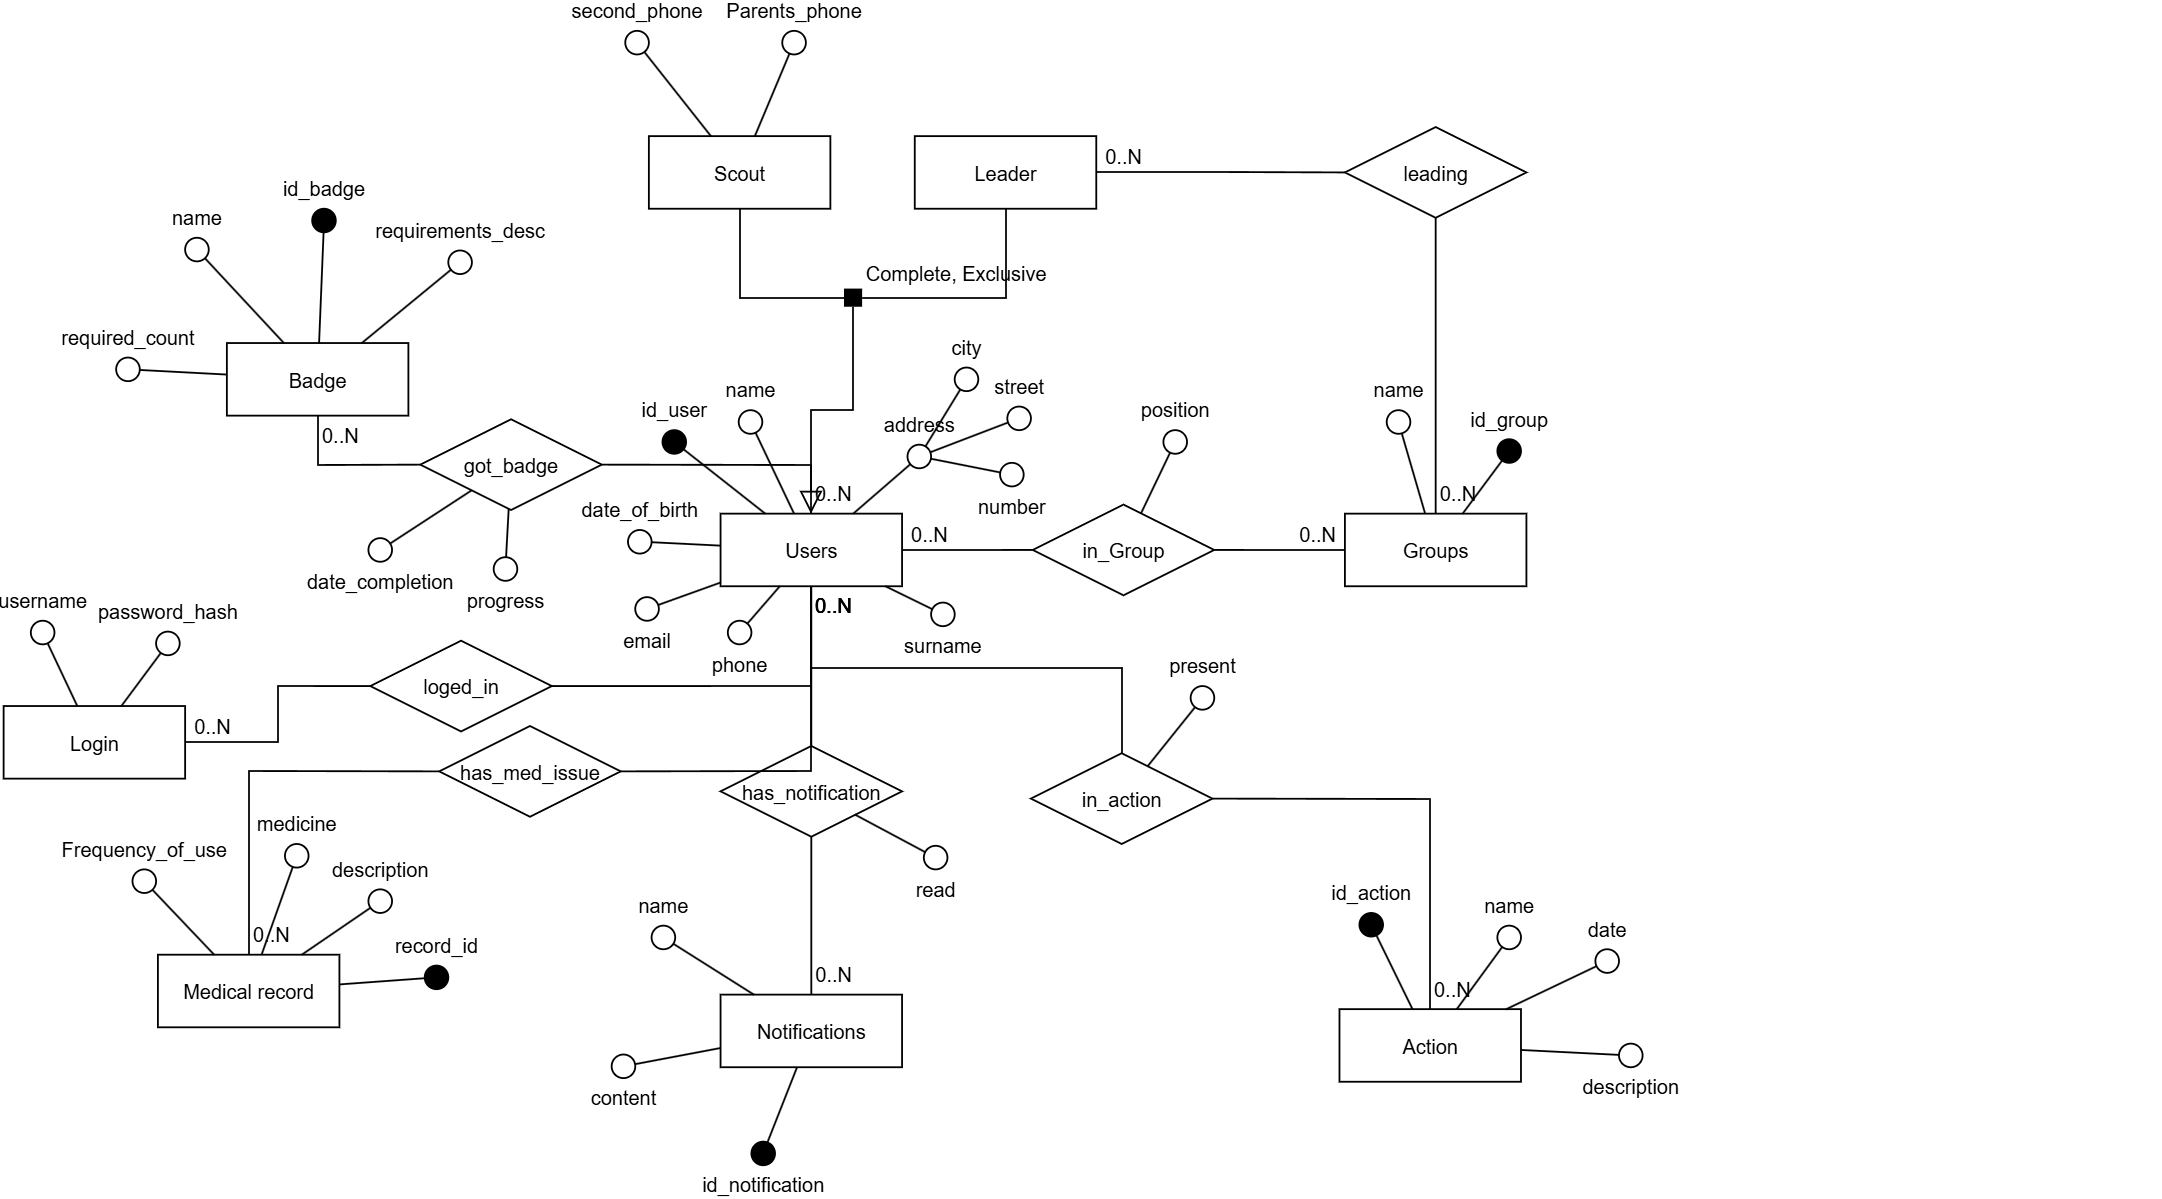
\includegraphics[width=1.5\linewidth]{images/er_diagram.png}
    \caption{ER diagram databáze}
    \label{fig:er_diagram}
\end{figure}


\section{Reálné využití}
Pro příklad reálného využití předpokládáme následující scénář. Vedoucí skautského oddílu má na starost 10 mladých skautů a chtěl by pro ně zorganizovat výlet do přírody. Při zavedení aplikace si všichni členové vytvořili své profily a nezletilí nechali své rodiče vyplnit své osobní údaje. Vedoucí oddílu vytvoří v aplikaci akci, kam vyplní všechny potřebné informace o místě setkání a věcech, které mají mít skauti s sebou. Každý skaut obdrží oznámení ve své aplikaci o nadcházející akci. Takové akce se plánují dostatečně dopředu, a proto se předpokládá, že během prvních pár dní si aplikaci otevře každý skaut, aby se o akci dozvěděl, nebo se to dozví na pravidelných schůzkách.

V den samotné akce si vedoucí může vytisknout papír s tabulkou pro vyplnění docházky. Má tak lepší přehled, které skauty má ten den na starost. Během akce se podaří některým skautům získat bobříky za výjimečné činnosti. Večer toho dne je může vedoucí zapsat do aplikace. Zde ani nevadí, že aplikace je pouze pro stolní počítače a notebooky, protože během výletu v přírodě nemusí být signál a vedoucí by tak musel se zapsáním bobříků stejně počkat.


\chapter{Závěr}
\section{Shrnutí}
Tato práce se zaměřila na analýzu a návrh aplikace pro správu skautského oddílu, která řeší potřeby vedoucích i skautů. Byly zhodnoceny existující aplikace, jako jsou SkautLS, Levitio, TroopTrack nebo Scoutbook. Na základě jejich nedostatků nebo nevyhovujících funkcionalitách byl vytvořen návrh nové aplikace. Návrh aplikace zahrnuje přehledné uživatelské rozhraní, možnost plánování akcí, administraci členů, správu bobříků, akcí, export dat a správu osobních údajů. Je zde zahrnut také informační systém pro efektivní šíření zpráv mezi vedoucími a skauty.


\section{Možná vylepšení}
Při vývoji aplikace se budou brát v potaz následující možná vylepšení:

\begin{itemize}
\item \textbf{Správa financí}

Přidání funkcí pro evidenci příjmů a výdajů oddílu, včetně možnosti sledovat platby za akce nebo tábory a spravovat rozpočet střediska.
\item \textbf{Propojení s osobním kalendářem}

Integrace aplikace s osobními kalendáři jako je Google Calendar. Díky tomu by si každý mohl přidat akce do svého mobilního zařízení a zmenšila se šance jejich zapomenutí.
\item \textbf{Zasílání informací na e-mail}

Možnost nastavení duplicitního zasílání oznámení na osobní e-mail.
\item \textbf{Podpora mobilních zařízení}

Úprava aplikace pro podporu systému Android. Ostatní systémy jako IoS vyžadují kompletní vývoj celé aplikace od začátku a proto nebudou součástí této práce.
\item \textbf{Offline režim}

Možnost používání aplikace bez připojení k internetu představuje bezpečnostní rizika. Využití této vlastnosti by opět mělo význam pouze pro mobilní zařízení.
\end{itemize}

\chapter{Zdroje}
\begin{itemize}

\item Skautské bobříky c2005–2024 [cit. 12.11.2024] \\
\url{https://foglarweb.skauting.cz/clanky.php?id=108}
\item FOGLAR, Jaroslav. Hoši od Bobří řeky. Praha: Olympia, 2005
\item Skauting c2024 [cit. 28.10.2024] \\
\url{https://cs.wikipedia.org/wiki/Skauting}
\item Historie skautingu c2024 [cit. 2.11.2024] \\
\url{https://www.skaut.cz/skauting/historie/}
\item SkautLS testovací stránka c2009-2024 [cit. 12.11.2024] \\
\url{https://test-is.skaut.cz/}
\item TroopTrack c2024 [cit. 13.11.2024] \\
\url{https://trooptrack.com/}
\item Scoutbook c2024 [cit. 13.11.2024] \\
\url{https://www.scouting.org/resources/scoutbook/}
\item Levitio c2024 [cit. 12.11.2024] \\
\url{https://www.levitio.cz/}
\item Rozdělení skautského sdružení c2024 [cit 8.12.2024] \\
\url{https://krizovatka.skaut.cz/organizace/organizacni-struktura}
\item jazyk Python c2001-2024 [cit. 9.12.2024] \\
\url{https://www.python.org/}
\item jazyk C++ c2024 [cit. 9.12.2024] \\
\url{https://en.wikipedia.org/wiki/C%2B%2B}
\item framework Qt6 c2024 [cit. 9.12.2024] \\
\url{https://www.qt.io/product/framework}
\item framework .NET c2024 [cit. 9.12.2024] \\
\url{https://dotnet.microsoft.com/en-us/}
\item databáze MySQL c2024 [cit. 9.12.2024] \\
\url{https://cs.wikipedia.org/wiki/SQL} \\
\url{https://www.mysql.com/}


\end{itemize}

\end{document}


% TODO
% tisk osobních údajů na výlety
% podpora angličtina/čeština